\documentclass[12pt,letterpaper]{article}
\usepackage{graphicx,textcomp}
\usepackage{natbib}
\usepackage{setspace}
\usepackage{fullpage}
\usepackage{color}
\usepackage[reqno]{amsmath}
\usepackage{amsthm}
\usepackage{fancyvrb}
\usepackage{amssymb,enumerate}
\usepackage[all]{xy}
\usepackage{endnotes}
\usepackage{lscape}
\newtheorem{com}{Comment}
\usepackage{float}
\usepackage{hyperref}
\newtheorem{lem} {Lemma}
\newtheorem{prop}{Proposition}
\newtheorem{thm}{Theorem}
\newtheorem{defn}{Definition}
\newtheorem{cor}{Corollary}
\newtheorem{obs}{Observation}
\usepackage[compact]{titlesec}
\usepackage{dcolumn}
\usepackage{tikz}
\usetikzlibrary{arrows}
\usepackage{multirow}
\usepackage{xcolor}
\newcolumntype{.}{D{.}{.}{-1}}
\newcolumntype{d}[1]{D{.}{.}{#1}}
\definecolor{light-gray}{gray}{0.65}
\usepackage{url}
\usepackage{listings}
\usepackage{color}

\definecolor{codegreen}{rgb}{0,0.6,0}
\definecolor{codegray}{rgb}{0.5,0.5,0.5}
\definecolor{codepurple}{rgb}{0.58,0,0.82}
\definecolor{backcolour}{rgb}{0.95,0.95,0.92}

\lstdefinestyle{mystyle}{
	backgroundcolor=\color{backcolour},   
	commentstyle=\color{codegreen},
	keywordstyle=\color{magenta},
	numberstyle=\tiny\color{codegray},
	stringstyle=\color{codepurple},
	basicstyle=\footnotesize,
	breakatwhitespace=false,         
	breaklines=true,                 
	captionpos=b,                    
	keepspaces=true,                 
	numbers=left,                    
	numbersep=5pt,                  
	showspaces=false,                
	showstringspaces=false,
	showtabs=false,                  
	tabsize=2
}
\lstset{style=mystyle}
\newcommand{\Sref}[1]{Section~\ref{#1}}
\newtheorem{hyp}{Hypothesis}

\title{Problem Set 1}
\date{Due: October 8, 2026}
\author{Applied Stats/Quant Methods 1}

\begin{document}
	\maketitle
	
	\section*{Instructions}
	\begin{itemize}
	\item Please show your work! You may lose points by simply writing in the answer. If the problem requires you to execute commands in \texttt{R}, please include the code you used to get your answers. Please also include the \texttt{.R} file that contains your code. If you are not sure if work needs to be shown for a particular problem, please ask.
\item Your homework should be submitted electronically on GitHub.
\item This problem set is due before 23:59 on Thursday October 8, 2026. No late assignments will be accepted.
	\end{itemize}
	
	\vspace{1cm}
	\section*{Question 1: Education}

A school counselor was curious about the average of IQ of the students in her school and took a random sample of 25 students' IQ scores. The following is the data set:\\
\vspace{.5cm}

\lstinputlisting[language=R, firstline=36, lastline=36]{PS01_CVH.R}  


\vspace{1cm}

\begin{enumerate}
\item Find a 90\% confidence interval for the average student IQ in the school. 
(As a hint, you first need the mean and SD to create a CI.)

The data is ratio (continuous), the sample size is 25 thus a small sample size with an unknown standard deviation. For this reason a $t$-distribution is appropriate. The sampling method is randomization, and the school counselor is interested in estimating the population mean which could be either higher or lower than the sample mean. For a 90\% confidence interval, the remaining 10\% is divided equally between the two tails, with 5\% in each tail.
\lstinputlisting[language=R, firstline=39, lastline=56]{PS01_CVH.R}	
\[
\begin{array}{c|c}
	\text{lower} & \text{upper} \\
	\hline
	93.96 & 102.92
\end{array}
\]
The 90\% confidence interval is 93.96 to 102.92, thus we are 90\% confident that the population mean IQ of students at the school is between the lower and upper limits of the confidence interval.

	\item Next, the school counselor was curious  whether  the average student IQ in her school is higher than the average IQ score (100) among all the schools in the country.\\ 
	\noindent Using the same sample, conduct the appropriate hypothesis test with $\alpha=0.05$.

The assumptions above are still applicable except this is a right-tailed test. The Null Hypothesis is that average IQ in the school is less than or equal to the national average. The Alternative Hypothesis is that the average IQ in the school is higher than the national average.
\[
\begin{aligned}
	H_0 &: \mu \leq 100 \\
	H_1 &: \mu > 100
\end{aligned}
\]
	\lstinputlisting[language=R, firstline=60, lastline=64]{PS01_CVH.R}	
If the p-value < 0.05, reject H0; otherwise, fail to reject H0. The p-value = 0.7215 thus at the 5\% significance level, there is insufficient evidence to conclude that the average student IQ is greater than 100. We fail to reject the H0.
\end{enumerate}

\newpage

	\section*{Question 2: Political Economy}

\noindent Researchers are curious about what affects the amount of money communities spend on addressing homelessness. The following variables constitute our data set about social welfare expenditures in the USA. \\
\vspace{.5cm}


\begin{tabular}{r|l}
	\texttt{State} &\emph{50 states in US} \\
	\texttt{Y} & \emph{per capita expenditure on shelters/housing assistance in state}\\
	\texttt{X1} &\emph{per capita personal income in state} \\
	\texttt{X2} &  \emph{Number of residents per 100,000 that are "financially insecure" in state}\\
	\texttt{X3} &  \emph{Number of people per thousand residing in urban areas in state} \\
	\texttt{Region} &  \emph{1=Northeast, 2= North Central, 3= South, 4=West} \\
\end{tabular}

\vspace{.5cm}
\noindent Explore the \texttt{expenditure} data set and import data into \texttt{R}.
\vspace{.5cm}
\lstinputlisting[language=R, firstline=42, lastline=42]{PS01_CVH.R}  
\vspace{.5cm}
\begin{itemize}

\item
Please plot the relationships among \emph{Y}, \emph{X1}, \emph{X2}, and \emph{X3}? What are the correlations among them (you just need to describe the graph and the relationships among them)?
	\lstinputlisting[language=R, firstline=77, lastline=112]{PS01_CVH.R}
\text The scatterplot (Figure 1) matrix shows upward-sloping patterns between all pairs of variables, consistent with their positive correlations. The correlation shows X1 has the strongest relationship with Y, followed by X3 and X2 (Table 1 and 2).
	
\vspace{.5cm}
\item
Please plot the relationship between \emph{Y} and \emph{Region}? On average, which region has the highest per capita expenditure on housing assistance?
	\lstinputlisting[language=R, firstline=121, lastline=135]{PS01_CVH.R}
Figure 2 shows that the second boxplot (North Central) has the most outliers and the fourth boxplot (West) has the longest upper and lower whisker. The West (Region 4) has the highest average expenditure, with a average mean of 88.31 per capita. The North Central region (Region 2) has the second-highest average at 83.92, followed by the Northeast (Region 1) at 79.44. The South (Region 3) has the lowest average expenditure at 69.19 per capita (Table 3).
	
\vspace{.5cm}
\item
Please plot the relationship between \emph{Y} and \emph{X1}? Describe this graph and the relationship. Reproduce the above graph including one more variable \emph{Region} and display different regions with different types of symbols and colors.
	\lstinputlisting[language=R, firstline=142, lastline=156]{PS01_CVH.R}
The scatterplot shows a moderate positive relationship between X1 and Y:as per-capita personal income (X1) increases, per-capita expenditure on housing assistance (Y) generally increases. The correlation between the two variables is 0.532, indicating a moderate positive linear association (Table 2). 

The abline's formula is Y = 32.546 + 0.02458X\_1. Approximately 28.27\% of the variation in Y is explained by X1 using this linear regression model.
\lstinputlisting[language=R, firstline=160, lastline=176]{PS01_CVH.R}
There is a positive relationship, as per-capita personal income increases, housing-assistance expenditure generally tends to increase. This relationship is not very strong nor perfectly linear. Therefor income alone does not explain differences in housing-assistance expenditure and there are big differences (Figure 4).
	
\end{itemize}
\newpage
\begin{center}
	\Large\textbf{Bibliography}
\end{center}

\noindent Statistics Resources: Correlation. (2026, September 29). Retrieved from National University: \url{https://resources.nu.edu/statsresources/correlation}
```
\newpage
	\section*{Figures and Tables}
\begin{figure}[h]
	\centering
	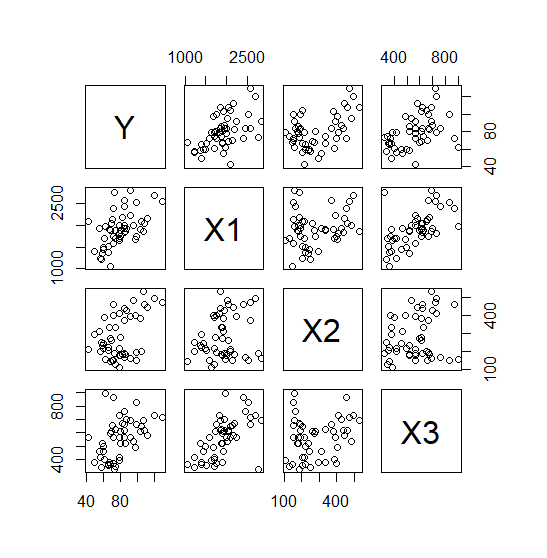
\includegraphics[width=0.7\textwidth]{PNG Files/Correlation_plot.png}
	\caption{Correlation Matrix of Y, X1, X2, and X3}
	\label{fig:correlation}
\end{figure}
\begin{table}[htbp]
	\centering
	\caption{Correlation Matrix of the Dependent and Independent Variables}
	\label{tab:correlation_matrix}
	\[
	\begin{array}{c|rrrr}
		& Y & X_1 & X_2 & X_3 \\ \hline
		Y   & \text{NA} & 0.5317 & 0.4483 & 0.4637 \\
		X_1 & 0.5317 & \text{NA} & 0.2056 & 0.5953 \\
		X_2 & 0.4483 & 0.2056 & \text{NA} & 0.2210 \\
		X_3 & 0.4637 & 0.5953 & 0.2210 & \text{NA}
	\end{array}
	\]
\end{table}
\vspace{2cm}
\begin{table}[htbp]
	\centering
	\caption{Classification of Correlation Strengths}
	\label{tab:correlation_strength}
	\[
	\begin{array}{c|c|c|c|c}
		& Y & X_1 & X_2 & X_3 \\ \hline
		Y   & \text{NA} & \text{Moderate Positive} & \text{Moderate Positive} & \text{Moderate Positive} \\
		X_1 & \text{Moderate Positive} & \text{NA} & \text{Weak Positive} & \text{Moderate Positive} \\
		X_2 & \text{Moderate Positive} & \text{Weak Positive} & \text{NA} & \text{Weak Positive} \\
		X_3 & \text{Moderate Positive} & \text{Moderate Positive} & \text{Weak Positive} & \text{NA}
	\end{array}
	\]
\end{table}

\begin{figure}[h]
	\centering
	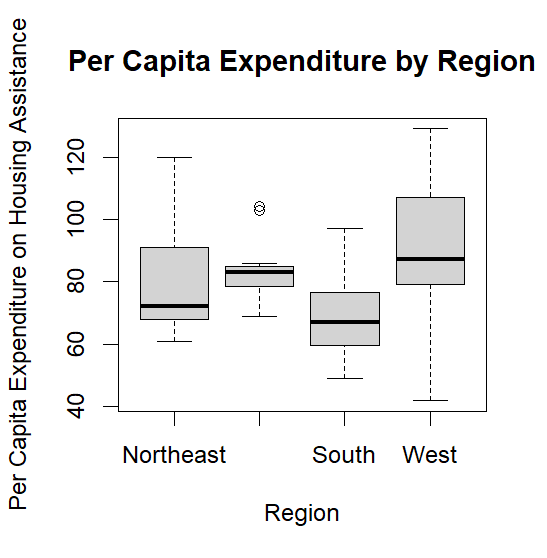
\includegraphics[width=0.7\textwidth]{PNG Files/Boxplot_region.png}
	\caption{Average Per Capita Expenditure on Housing Assistance by Region}
	\label{fig:correlation}
\end{figure}

\begin{table}[htbp]
	\centering
	\caption{Mean Per-Capita Expenditure on Shelters and Housing Assistance by Region}
	\label{tab:expenditure_by_region}
	\[
	\begin{array}{c|c}
		\text{Region} & \text{Mean } Y \\ \hline
		\text{Northeast} & 79.44444 \\
		\text{North Central} & 83.91667 \\
		\text{South} & 69.18750 \\
		\text{West} & 88.30769
	\end{array}
	\]
\end{table}

\begin{figure}[h]
	\centering
	\includegraphics[width=0.7\textwidth]{PNG Files/Relationship_y_x1.png}
	\caption{Scatter-plot of Y and X1}
	\label{fig:correlation}
\end{figure}

\begin{figure}[h]
	\centering
	\includegraphics[width=0.7\textwidth]{PNG Files/Relationship_y_x1_region.png}
	\caption{Scatter-plot of Y and X1 by Region}
	\label{fig:correlation}
\end{figure}


\end{document}
